\subsection{Sufficient conditions of goodness}

\subsubsection{Results}

A horizontal rectangle $\D$ is good, if
\begin{equation}\label{goodness_condition}
	\dfrac{\D_1}{\D_2} <
	\left\{\begin{array}{ll}
		3.8, & i_1 \equiv i_2 \pmod 2,\\
		3.43, & i_1 \not\equiv i_2 \pmod 2.
	\end{array}\right.
\end{equation}

\subsubsection{Universal $2,9$ bound}

Now let's introduce some sufficient conditions for rectangle to be good.

Remind that we suppose $|\D_1| \geqslant |\D_2|$, which means that

\begin{equation*}
	q
	\dfrac{1 + p \T_{1}}{1 + p' \T_{1}}
	\dfrac{1 + p \T_{95}}{1 + p' \T_{95}} \leqslant 1.
\end{equation*}

Let's introduce the following designations:
\begin{equation*}
	\g = [0; a_{-1}, ..., a_{i_1}, \frac{1}{\T_\g}],
\end{equation*}
\begin{equation*}
	\d = [0; a_{1}, ..., a_{i_2}, \frac{1}{\T_\d}],
\end{equation*}

where $\T$'s are some $\T$'s from the Figure \oldref{fg:table-thetas},
specified in each case separately.

\begin{figure}[p]
	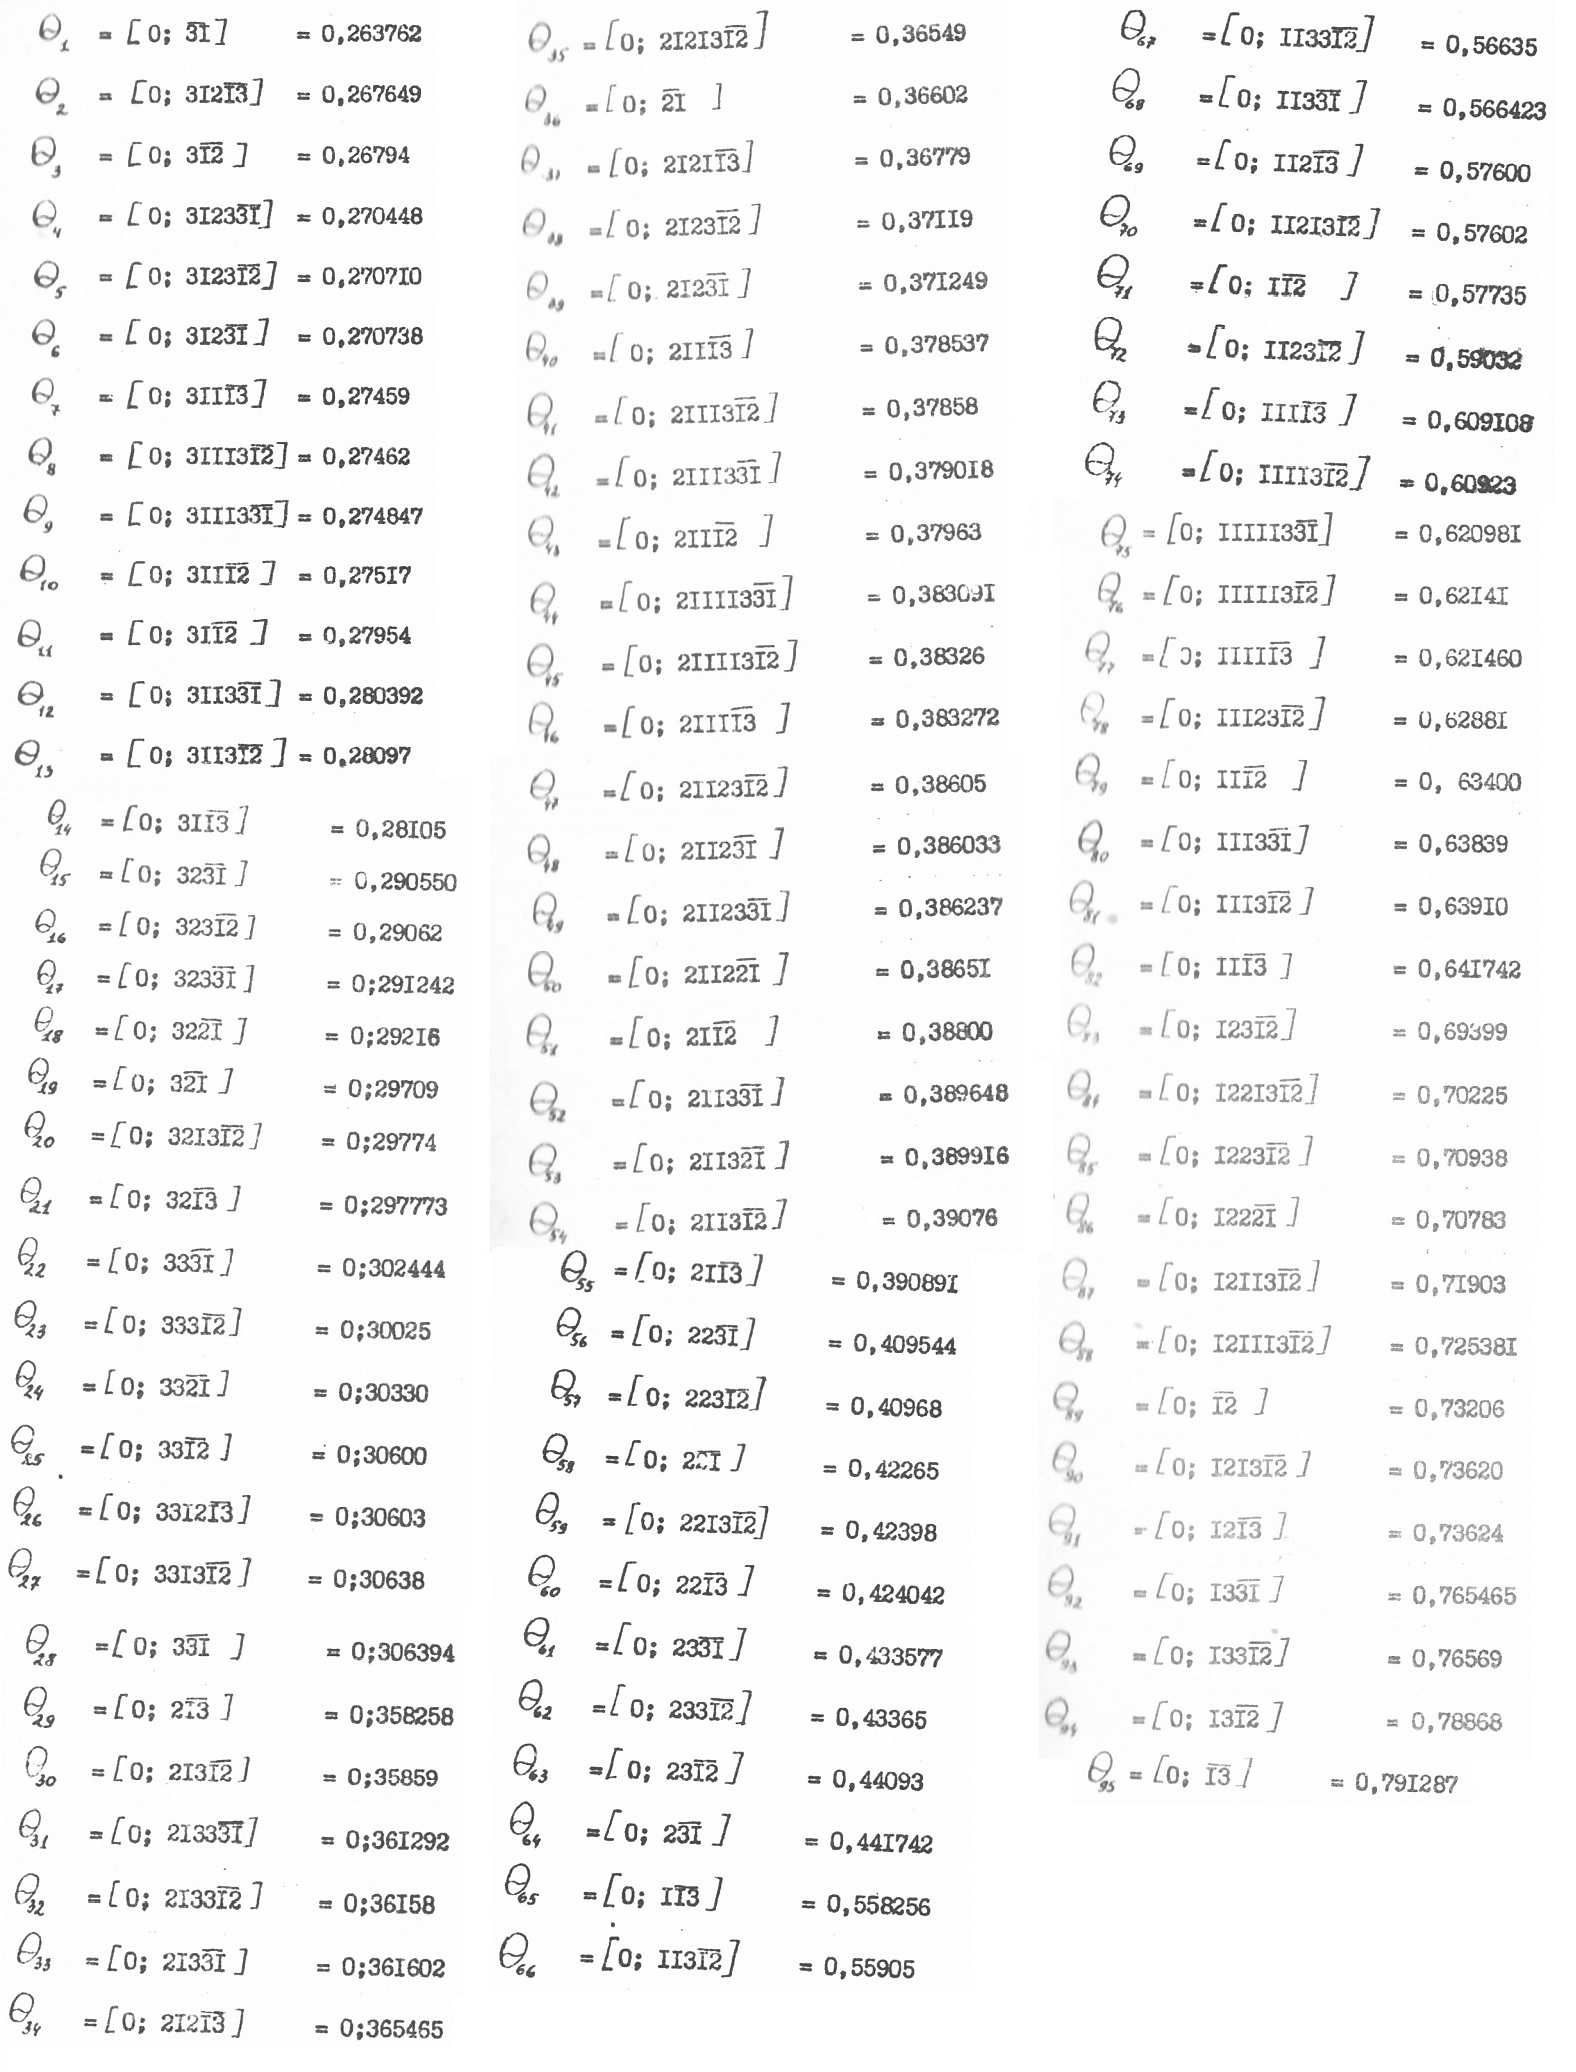
\includegraphics[width=\textwidth]{table-thetas}
	\caption{List of $\T$'s.}
	\label{fg:table-thetas}
\end{figure}

If rectangle is good, then \ref{goodness_in_deltas} should take place:

\begin{equation}\label{goodness_in_deltas}
	\g' - \g'' < |\d' - \d''|,
\end{equation}

where
$\T_{\g'} = \T_{66}$,
$\T_{\g''} = \T_{63}$,
$\T_{\d'} = \T_{90}$,
$\T_{\d''} = \T_{30}$.

Inequality \ref{goodness_in_deltas} transforms into

\begin{equation}\label{12.2}
	0,313 <
	q
	\dfrac{1 + p \T_{63}}{1 + p' \T_{30}}
	\dfrac{1 + p \T_{66}}{1 + p' \T_{90}}.
\end{equation}

Suppose that

\begin{equation}\label{goodness_condition_2,9}
	\dfrac{\D_1}{\D_2} < 2,9,
\end{equation}

which is equivalent to

\begin{equation}
	\dfrac{1}{q}
	\dfrac{1 + p' \T_{1}}{1 + p \T_{1}}
	\dfrac{1 + p' \T_{95}}{1 + p \T_{95}}
	<
	2,9.
\end{equation}

Then \ref{12.2} takes place. Indeed, it is so, if

\begin{equation*}
	\dfrac{1}{2,9}
	\dfrac{1 + p' \T_{1}}{1 + p \T_{1}}
	\dfrac{1 + p' \T_{95}}{1 + p \T_{95}}
	>
	0,313
	\dfrac{1 + p' \T_{30}}{1 + p \T_{63}}
	\dfrac{1 + p' \T_{90}}{1 + p \T_{66}}.
\end{equation*}

or, equivalent,

\begin{equation*}
	1,1
	>
	\dfrac{1 + p \T_{1}}{1 + p \T_{63}}
	\dfrac{1 + p \T_{95}}{1 + p \T_{66}}
	\dfrac{1 + p' \T_{30}}{1 + p' \T_{1}}
	\dfrac{1 + p' \T_{90}}{1 + p' \T_{95}},
\end{equation*}

which is checked directly.

Condition \ref{goodness_condition_2,9} is sufficient for rectangle to be good,
regardless of the parity of $i_1$ and $i_2$ and the left or right shortness or normalness of rectangle.

\subsubsection{Case $i_1 = i_2 \pmod 2$}

Now consider case $i_1 = i_2 \pmod 2$.

\pic[0.5]{pic4}

We will suppose case $a_{i_2} = 1$, $a_{i_2 - 1} = 3$ doesn't take place.

We can substitute the folliwing $\g$'s and $\d$'s
into \ref{goodness_in_deltas}:

\Ts{66}{63}{90}{3}

and instead of \ref{12.2} we will get

\begin{equation}\label{12.5}
	0,253 < q
	\dfrac{1 + p \T_{63}}{1 + p' \T_{3}}
	\dfrac{1 + p \T_{66}}{1 + p' \T_{90}}.
\end{equation}

This choose of $\T_{\g'}$ and $\T_{\d''}$ is fine,
if the following inequality takes place:

\begin{equation}\label{goodness_condition_1,4}
	\d' - \d'' > 1,4 (\g' - \g''),
\end{equation}

where 
\begin{equation*}
	\T_{\g'} = \T_{68},\;
	\T_{\g''} = \T_{65},\;
	\T_{\d'} = \T_{28},\;
	\T_{\d''} = \T_{1},
\end{equation*}

so we can rewrite \ref{goodness_condition_1,4} as

\begin{equation}\label{12.7}
	0,253 < q
	\dfrac{1 + p \T_{65}}{1 + p' \T_{1}}
	\dfrac{1 + p \T_{68}}{1 + p' \T_{28}}.
\end{equation}

We can notice that \ref{12.7} follows from \ref{12.5}. Indeed, that follows from the inequality

\begin{equation*}
	0,253
	\dfrac{1 + p' \T_{3}}{1 + p' \T_{63}}
	\dfrac{1 + p \T_{90}}{1 + p \T_{66}}
	>
	0,269
	\dfrac{1 + p' \T_{1}}{1 + p' \T_{65}}
	\dfrac{1 + p \T_{28}}{1 + p \T_{68}},
\end{equation*}

or inequality

\begin{equation*}
	\dfrac{1 + p \T_{65}}{1 + p \T_{63}}
	\dfrac{1 + p \T_{68}}{1 + p \T_{66}}
	\dfrac{1 + p' \T_{3}}{1 + p' \T_{1}}
	\dfrac{1 + p' \T_{90}}{1 + p' \T_{28}}
	>
	1,064.
\end{equation*}

Overall, we proved that \ref{12.5} is enough for rectangle to be good.

Suppose that

\begin{equation}\label{goodness_condition_3,8}
	\dfrac{\D_1}{\D_2} < 3,8,
\end{equation}

or

\begin{equation*}
	\dfrac{1}{q}
	\dfrac{1 + p' \T_{1}}{1 + p \T_{1}}
	\dfrac{1 + p' \T_{95}}{1 + p \T_{95}}
	<
	3,8.
\end{equation*}

Then \ref{12.5} takes place. Indeed, it is so, if

\begin{equation*}
	\dfrac{1}{3,8}
	\dfrac{1 + p' \T_{1}}{1 + p' \T_{1}}
	\dfrac{1 + p \T_{95}}{1 + p \T_{95}}
	>
	0,253
	\dfrac{1 + p' \T_{3}}{1 + p' \T_{63}}
	\dfrac{1 + p \T_{90}}{1 + p \T_{66}}.
\end{equation*}

The last inequality is transformed into

\begin{equation*}
	1,04
	>
	\dfrac{1 + p' \T_{3}}{1 + p' \T_{1}}
	\dfrac{1 + p' \T_{90}}{1 + p' \T_{95}}
	\dfrac{1 + p \T_{1}}{1 + p \T_{63}}
	\dfrac{1 + p \T_{95}}{1 + p \T_{66}},
\end{equation*}

which is easily checked.

\subsubsection{Case $i_1 \ne i_2 \pmod 2$}

Now consider case $i_1 \ne i_2 \pmod 2$
and, again, case $a_{i_2} = 1$, $a_{i_2 - 1} = 3$
doesn't take place.
Suppose that $i_1$ is even.

\pic[0.6]{pic5}

Taking
\begin{equation*}
	\T_{\g'} = \T_{66},\;
	\T_{\g''} = \T_{59},\;
	\T_{\d'} = \T_{3},\;
	\T_{\d''} = \T_{90},
\end{equation*}

rewrite \ref{goodness_in_deltas} as

\begin{equation}\label{12.9}
	0,2885
	<
	q
	\dfrac{1 + p \T_{59}}{1 + p' \T_{3}}
	\dfrac{1 + p \T_{66}}{1 + p' \T_{90}}.
\end{equation}

Suppose

\begin{equation}\label{goodness_condition_3,43}
	\dfrac{\D_1}{\D_2} < 3,43
\end{equation}

or

\begin{equation*}
	\dfrac{1}{q}
	\dfrac{1 + p' \T_{1}}{1 + p \T_{1}}
	\dfrac{1 + p' \T_{95}}{1 + p \T_{95}}
	<
	3,43.
\end{equation*}

Then \ref{12.9} takes place. Indeed, it is so, if

\begin{equation*}
	\dfrac{1}{3,43}
	\dfrac{1 + p' \T_{1}}{1 + p \T_{1}}
	\dfrac{1 + p' \T_{95}}{1 + p \T_{95}}
	>
	0,2885
	\dfrac{1 + p' \T_{3}}{1 + p \T_{59}}
	\dfrac{1 + p' \T_{90}}{1 + p \T_{66}}.
\end{equation*}

or

\begin{equation*}
	1,0105
	>
	\dfrac{1 + p' \T_{3}}{1 + p' \T_{1}}
	\dfrac{1 + p' \T_{90}}{1 + p' \T_{95}}
	\dfrac{1 + p \T_{1}}{1 + p \T_{59}}
	\dfrac{1 + p \T_{95}}{1 + p \T_{66}},
\end{equation*}

increasing the right part, obtain

\begin{equation*}
	1,0105
	>
	0,9896
	\dfrac
	{1 + p \cdot 1,0551 + p^2 \cdot 0,20875}
	{1 + p \cdot 0,983 + p^2 \cdot 0,237},
\end{equation*}

which is easily checked.
